
%%% Local Variables:
%%% mode: latex
%%% TeX-master: t
%%% End:

\chapter{基于AS编址的互联网可扩展路由机制框架}
\label{cha:model}

\section{引言}
    本章将详细描述基于AS的无类编址方案CABA,以及在此编址方案下采用的基于AS号的域间路由机制A-BGP。

\section{基于AS的无类编址方案}

\begin{table}[h]
    \centering
    \caption{CABA:基于ASN的地址分配方案}
    \label{tab:caba}
        \begin{tabular}{|c|c|c|c|}
        \hline
        8 & 32 & 24 & 64\\ \hline
        Res & ASN & subnet ID & interface ID\\ \hline
        保留位& 域间可路由前缀 & 域内可路由前缀 & 接口ID\\
        \hline
        \end{tabular}
\end{table}

本文的仿真与测试实验基于一种新型的基于AS编址的层次化编址方案CABA,其编址方案如图\ref{tab:caba}所示:

该编址方案前8位为保留位,即该方案目前只使用了整个IPv6地址的$1/256$,为以后IPv6地址可能出现的其他情况做好准备。从网络层次结构分析,该编址方案为层次化的编址结构,将IPv6 地址空间分为域间的AS 域,域内的子网域和接口ID,以此来分离域内和域间路由,可有效减少域内路由振荡对域间路由的影响。从地址聚合的角度分析,域间使用AS进行聚合,域内使用IP 前缀进行聚合,可能目前域间AS 聚合难度较大,但是域内IP 前缀聚合发展已经较为成熟。


关于域间AS聚合的问题,我们了解到目前对自治系统号的定义为32位,目前全球有5万多个AS,而32bits可以分配4294967296个自治系统号,未来将分配更多的自治系统号,在分配的过程中可以考虑分配给互连的自治系统可以聚合的自治系统号。这样AS域可以分为两大类,一类是不需要聚合的顶级服务提供商使用的自治系统域,另一类是可以聚合的非顶级的服务提供商使用的自治系统域。


域间路由采用基于自治系统号的BGP外部网关协议;域内路由24位仍可参考IPv4的内部网关协议,兼容现今网络。

IPv4中0.0.0.0为默认网络,在该IPv6中0::0可以作为默认网络。

\section{基于自治系统号的BGP协议}

基于自治系统号的域间路由协议,将自治系统号作为域间路由的前缀。因为自治系统的变化是小概率事件,且域间路由与域内路由使用不同的地址段,相互独立,域内路由振荡不会影响域间路由,所以极大减少了路由通告的数量,压缩了域间全局路由表,提高了路由的可扩展性。原本一个自治系统可能宣告多个前缀,但在基于自治系统号的BGP协议中一个自治系统只需向外宣告一个前缀。同时,自治系统的多个前缀发生变动的概率远大于自治系统号改变的概率,所以在该基于自治系统号的BGP 协议中,路由振荡的频率会减少。

\begin{figure}
  \centering
  % Requires \usepackage{graphicx}
  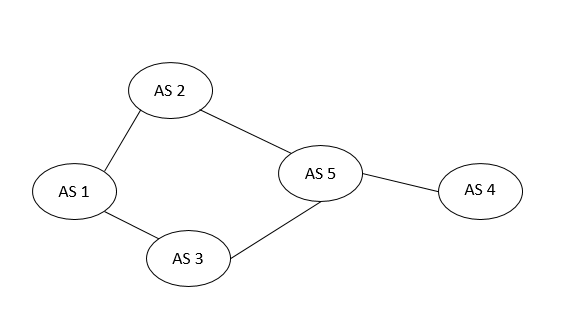
\includegraphics[width=\textwidth]{abgpexample}
  \caption{基于ASN-BGP路由示例-AS关系图}
  \label{fig:abgpexample}
\end{figure}


基于自治系统号的BGP协议域间路由的示例如下,自治系统之间的关系如图\ref{fig:abgpexample}:

\begin{itemize}
\item 自治系统4发布AS4$/$32的路由前缀,自治系统5收到自治系统4的通告,自治系统5的自治系统号可以和自治系统4的自治系统号相聚合,所以自治系统5将收到的路由信息进行聚合。
\item 自治系统5发布聚合后的AS4$/$31和详细路由AS4$/$32,自治系统2和自治系统3收到来自自治系统5的通告。
\item 自治系统2和3分别发布聚合后的AS4$/$31和详细路由AS4$/$32,自治系统1分别收到来自自治系统2和3的通告,共4条。

\begin{table}[h]
    \centering
    \caption{自治系统收到的路由信息}
    \label{tab:oneroutinginfo}
        \begin{tabular}{|c|c|c|c|}
        \hline
            路由信息编号 & AS前缀 & 下一跳 & AS路径\\ \hline
            路由信息1 & AS4$/$32 & 自治系统2 & 2,5,4\\ \hline
            路由信息2 & AS4$/$32 & 自治系统3 & 3,5,4\\ \hline
            路由信息3 & AS4$/$31 & 自治系统2 & 2,5\\ \hline
            路由信息4 & AS4$/$31 & 自治系统3 & 3,5\\
        \hline
        \end{tabular}
\end{table}
    如上图\ref{tab:oneroutinginfo},基于AS的路由聚合算法,选择前缀更短的路由,则路由信息3和4可作为可选路由。如果是单路径机制,选择下一跳ASN 较小的路径,则路由信息3作为自治系统1的最佳路径。如果是多路径机制,最多选择两个非相交的路径,则路由信息3和4作为自治系统1的最佳路径。

\end{itemize}



基于自治系统号的BGP协议支持现有的通告IP前缀的路由协议,因此CABA编址方式可以在网络中进行增量部署。在自治系统部署了CABA编址的情况下,如果其邻居也部署了CABA编址,则基于自治系统号的BGP协议向邻居宣告基于ASN的前缀路由信息,如果其邻居没有部署CABA编址,则基于自治系统号的BGP协议向邻居宣告原有的IP前缀路由信息。

\section{小结}
通过了解基于AS编址的互联网可扩展路由机制框架,我们了解到基于AS编址的CABA将网络明确地划分成域内和域间两个层级,域内和域间路由的振荡相互独立,全局路由表中只有域间自治系统路由的信息,且每个自治系统仅向外公布一条嵌入自治系统号的前缀,可以合理推测基于AS 的编址CABA能有效减小路由表的大小和路由表的更新频率,提升路由的可扩展性。

